% TODO go back and rewrite the abstract


\documentclass{report}
\usepackage[utf8]{inputenc}
\usepackage{cite}
\usepackage{amsfonts}
\usepackage{amsmath}
\usepackage{mathtools}
\usepackage{algorithm, algpseudocode}
\usepackage{hyperref}
\usepackage{amssymb}
\usepackage{graphicx}
\graphicspath{{../pdf/}{D:}}


\title{Collaborative Filtering using K Nearest Neighbors}
\date{December\\ 2018}
\author{Michael Siem \\ \href{mailto:siem@wisc.edu}{siem@wisc.edu}
	\and Nathan Weinshenker \\ \href{mailto:nweinshenker@wisc.edu}{nweinshenker@wisc.edu}
	\and Jack Long \\ \href{mailto:jlong25@wisc.edu}{jlong25@wisc.edu}}

\begin{document}

\maketitle

\chapter*{Abstract}
Recommendation systems are a vital tool for providing users with personalized suggestions for items such as movies, music, and restaurants.
Product review data is widely accessible on services such as Spotify, Amazon, and Yelp.
There are two approaches that can be used to make recommendations to users based on this data, memory based, and model based.
Model based systems rely on approximating the data and determining features that are most likely to influence a users rating on an item. 
Matrix Decomposition methods such a SVD are an example of a model based system used to provide recommendations.
Over time models can become outdated and need to be updated to provide a more accurate recommendation.
Memory based systems rely upon maintaining data and finding users or items that are similar to each other.
The advantage of a memory based system is it doesn't learn a model or make any assumptions about the data so if trends change the recommendation system will adapt.
Memory based systems can do a user-user comparison or and item-item comparison.
In the user-user comparison, a user is compared to other users that have rated an item and in the item-item comparison, an item is compared to other items a user has rated to predict the rating the user will give it.
We will further study a memory based recommendation systems, K Nearest Neighbors. After this activity, you should have a firm understanding of how K Nearest Neighbors is affected by 1) choosing different K values; 2)adding more features to our feature matrix; 3) evaluating different distance functions; and 4) changing the classification decision rule.

\chapter*{Background Information}
	
\section*{K Nearest Neighbors}
	
K Nearest Neighbors (k-NN) is a memory based collaborative filter that relies upon comparing features of a user or item to other users or items to receive a recommendation. 
k-NN is a simple and powerful tool that doesn't require advanced tuning methods. 
It is a "lazy" solution in the sense that it doesn't need to do any training\cite{1}.
Because k-NN relies on a large set of data, it is slow to run: O(md) where m = \# examples and d = \# dimensions.

\subsection*{History of Nearest Neighbors}

In 1992, Paul Resnick and fellow researchers at the University of Minnesota first studied collaborative filtering systems through the GroupLens project\cite{2}.  Collaborative filtering began to arise as a solution for dealing with overload in online information spaces. The first collaborative filtering system was built by developers at Tapestry who collected ratings from Usenet readers (an old messaging network for academia) and
used them to predict whether or not other readers would like an article before they read it.\cite{3} With the growth of the Internet, collaborative filters systems have grown in scope and popularity with big name tech companies like Netflix, Amazon, and Yahoo. Today, collaborative filtering systems are used by many companies to shift through the mountains of readily available data and develop robust recommendation systems.

\subsection*{K Nearest Neighbor Pseudocode }
\begin{algorithm}
  \caption{K Nearest Neighbour}
  \begin{algorithmic}
  	\State Classify (X,Y,x) // X:training data, Y: class labels of X, x:unknown sample
	\For{ t = 1 to T}
	\State Compute the distance between $d(X, x)$
	\State Sort all the distances in ascending order
	\EndFor
	\State Find the set Z containing indices for the k smallest distances $d(X_{i},x)$
	\State return the set of k closest points 
  \end{algorithmic}
\end{algorithm}
\textsubscript{Our pseudocode will serve as the map for our derivation.}

\subsection*{K}

The value of K determines how many points (determined by the distance function) to use to predict a value for a point of interest.
The value of K can be determined by considering a range of K values using the data in memory.
If K is too small, it will model the noise in the data set, and if K is too large, the neighbors will include points from other classes.
K is generally chosen to be odd so that a majority will exist in the neighbors.

\subsection*{The Distance Function}

Several methods can be used to evaluate the distances between the neighbors and the point of interest.
Distance relates to all the attributes and assumes all of them have the same effects on a distance.
If there are attributes included in the k-NN that are irrelevant, it can cause errors in the classification.
This is known as the curse of dimensionality. 

\paragraph*{Euclidean Distance}

\begin{equation}
d(x_{i},x_{j}) = \sqrt{(x_{i1} - x_{j1})^2 + (x_{i2} - x_{j2})^2 + ... + (x_{ip} - x_{jp})^2}
\end{equation}

\paragraph*{Manhattan Distance}

\begin{equation}
d(x_{i},x_{j}) = |(x_{i1} - x_{j1})| + |(x_{i2} - x_{j2})| + ... + |(x_{ip} - x_{jp})|
\end{equation}

\subsection*{Classification Decision Rule}

Once we have the k closest points to the point of interest, we must decide how to apply the labels of the k neighbors to the sample.
The most basic classifier is the majority classifier.

\paragraph{Majority Classifier}

\begin{equation}
R_i = mode(labels of K nearest neighbors),  
\end{equation}
$R_i$ = rating for sample i

\paragraph{Average Classifier}

The average classifier takes an average of the k nearest neighbors.

\begin{equation}
R_i = \sum_{k=1}^k L_i / K
\end{equation}
$L_i$ = label of sample i
\\
The majority classifier applies the most frequent label of the k neighbors to the point of interest. 

\subsection*{Nearest Neighbor Classification Derivation}

\paragraph*{Terminology and Notation }\cite{4}

\begin{enumerate}
	\item P(A $|$ B), the conditional probability, is the probability of A given B
	\item $h : X \in 0, 1$  \qquad  \qquad \textrm{binary classification rule; 
	"classifier" }
	\item \begin{equation*}
	  \textbf{A}_{h_(x) \neq y} = \begin{cases}
	        0 & h(x) = y 
	        \\ 
	        1 &  otherwise.
	        \end{cases} \qquad \textrm{Loss Function}
	 \end{equation*}
\end{enumerate}
Here, we define $X$ as training data; $Y$ as class labels; and $x$ as the unknown sample; and our distance metric $d$ as the Euclidean distance.
\\ \\
First, k-NN calculates the distances between all  training samples $X_{i}$ and $x$ and sorts all the distances according to:
\begin{equation}
d(x,x_{i}) <= d(x,x_{i+1})
\end{equation}
We then define $N$ as the set of k closest points such that:
\begin{equation}
N_{k}(x) = (x_{1}, y_{1}), (x_{2}, y_{2}), ... , (x_{k}, y_{k}) \qquad where \qquad k \in N
\end{equation} 
This is called a k-neighborhood of $x$  \\ \\
With $N$ as a ordered list of k closest points, we can determine the label of our sample point $x$ w.r.t the majority of classes among neighbors
\begin{equation*}
\hat{p}(Y = y | x) = \frac{1}{k} \sum_{1}^{n} \textbf{A}_{h_(x_{i}) \neq y} 
\end{equation*}
\begin{equation}
\hat{Y}(x) = argmax_{\hat{p}}(Y = y |x)
\end{equation}
Here we compute the percentage of points classified as either 1 or 0 in the neighborhood and take the most frequent class label as the new class label for $x$. \cite{5}
 \newline\newline
		
\subsubsection*{Error Analysis}

The accuracy of the recommendation system will be analyzed in 2 ways.
First we will look at the percent of miss-classified ratings.

\begin{equation}
	Accurary =  \frac{\sum miss classified users}{total N} * 100
\end{equation}

Second we will look at the Root Mean Squared Error of the predictions versus the actual rating. 
Root Mean Squared Error (RMSE) is a popular metric in recommendation systems.
It is useful to know the RMSE because in a recommendation system with ratings on a scale of 1 to 5 or 1 to 10, there is a higher probability for something to be miss-classified than in a binary classification. 
The RMSE takes into account how far off a prediction is.

\begin{equation}
RMSE = sqrt(\frac{\sum_{k=1}^n(R_{pred} - R_{actual})^2}{N})
\end{equation}

\section*{Warm-up}

\begin{enumerate}
  \item Below is a diagram of points with classifications of either Red Triangle or Blue Square. 
	\begin{figure}[H]
	  \centering
	  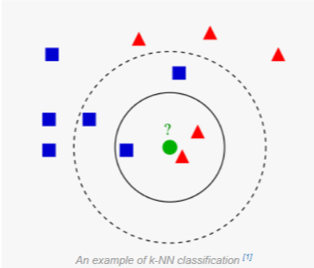
\includegraphics{image/Picture2.png}
	\end{figure}  
  	
  	\begin{enumerate}
  	  \item What is the classification of the green dot for the following k values using the majority classifier?
  	    \begin{center}
          \begin{tabular}{| l | l | l |}
            \hline
            k & Class \\ \hline
            1 & \\
            3 & \\
            5 & \\
			11 & \\            
            \hline
          \end{tabular}
        \end{center} 
        
        \item How does increasing k affect the performance in data sets with a lot of noise?
  	  \end{enumerate} 
  
  \item Use the table below to answer the following questions.
    \begin{center}
      \begin{tabular}{| l | l | l |}
        \hline
        Feature 1 & Feature 2 & Class \\ \hline
        -1 & 1 & - \\
        0 & 1 & + \\
        0 & 2 & - \\
        1 & -1 & - \\
        1 & 0 & + \\
        1 & 2 & + \\
        2 & 2 & - \\
        2 & 3 & + \\
        \hline
      \end{tabular}
    \end{center} 
  	
  	\begin{enumerate}
  	  \item Compute the Manhattan distance to a new point (1,1).
        \begin{center}
          \begin{tabular}{| l | l | l |}
            \hline
            Feature 1 & Feature 2 & Manhattan Distance \\ \hline
            -1 & 1 &  \\
            0 & 1 &  \\
            0 & 2 &  \\
            1 & -1 &  \\
            1 & 0 &  \\
            1 & 2 &  \\
            2 & 2 &  \\
            2 & 3 &  \\
            \hline
        \end{tabular}
      \end{center}
    
    \item Using the majority classifier, what is the label applied to the new point (1,1) for the following k-Values?
      \begin{center}
        \begin{tabular}{| l | l | l |}
          \hline
          k & Class \\ \hline
          1 & \\
          3 & \\
          4 & \\
          \hline
        \end{tabular}
      \end{center}       	  
  	\end{enumerate}

  \item Which of the following will be true both statements? \\

	1 - k-NN is a memory-based approach is that the classifier immediately adapts as we collect new training data. \\
	2 - The computational complexity for classifying new samples grows linearly with the number of samples in the training dataset in the worst-case scenario. \\ \\
		A) 1 \\
		B) 2 \\
		C) 1 and 2 \\
		D) None of these \\

\end{enumerate}

\chapter*{Main Activity}

The main activity will be evaluating a k-NN as a restaurant recommendation system using the Yelp dataset from \href{https://www.yelp.com/dataset}{https://www.yelp.com/dataset} using KNN.m and users.mat.
The dataset originally contains 5,996,996 reviews for 188,593 businesses in 10 metropolitan areas.
We preprocessed the data set to narrow it down to 1 restaurant and 500 reviews for the restaurant for the activity. The activity will be doing a user-user comparison to the users that have rated the restaurant.
The following features are available for use in the problem. 
The first 3 were taken directly from the user's profile, and the last 4 were derived from the users other reviews.

\begin{enumerate}
\item avg\textunderscore rating: The average rating the user has given to all businesses they have rated.
\item review\textunderscore count: The total number of reviews a user has given.
\item useful: Number of "useful" votes the user has given.
\item avg\textunderscore restaurant\textunderscore rating: The average rating the user has given to businesses classified as restaurants.
\item cats\textunderscore pizza: The number of businesses classified as a pizza restaurant the user has been to.
\item cats\textunderscore bar: The number of businesses classified as a bar the user as been to.
\item cats\textunderscore italian: The number of businesses classified as an Italian restaurant the user as been to.
\end{enumerate}

The restaurant being evaluated is Nora's Italian Cuisine. More details about the restaurant can be found in the comment near the top of KNN.m.

\section*{Problems}

\begin{enumerate}

\item Choosing K
  	
  	\begin{enumerate}
    
  	\item {
  	Run the file KNN.m to load all the variables. 
  	User ctrl+enter to run sections of the code to speed it up. 
  	Starting with all 7 features selected and k = 1.
  	What is the number of misclassified values and why is this (mind the few that show a difference of 1)?
  	}
  	
    \item {
   	Repeat the above for different values of k, how do the number of miss-classifications and RMSE vary with k? 
   	(You can change the k\textunderscore end variable to easily iterate over several values of k, but it will take a little time to run)
    }
    
	\end{enumerate}
	
\item {
Evaluating different features.
We will next evaluate the use of the different features available to reduce the number of features so that we are not suffering from the curse of dimensionality with all 7 of the features available. Call the plots.m to view classification groupings of 2 variables.
}

	\begin{enumerate}
	
	\item {	
	Select one feature from the features list to be used.
	To select the features, place the numbers for the corresponding features in the list features.
	Why is the error no longer zero for k = 1?
	}
	
	\item {
	Go to section Problem Choosing Features in the KNN.m file.
	Run this section of code with various K values.
	Which features seem to be best for classifying the data?
	}
	
	\end{enumerate}
	
\item {
Evaluating different distance functions.
Return to the Problem - Configuration and select a different distance function. 
Make sure to run this section after changing a variable to update it in the workspace.
}

	\begin{enumerate}
	
	\item {
	Set k equal to 3.
	Run the section Problem Choosing Features changing the distance metric each time in the Problem - Configuration section.
	Do the features all perform the same for the same distance metric?
	}
	
	\end{enumerate}


\item {
Evaluating different classification functions.
}
    \begin{enumerate}
	
	\item {
	Compare the majority classifier and the average classifier. How do they compare in number of missclassfied data and RMSE? 
	Use the sections Problem Choosing Features and Iteration over K for the Problem to evaluate.
	}    
    \end{enumerate}
    
\end{enumerate}

\begin {thebibliography}{999}
\bibliographystyle{plain}
	\bibitem{1}
	Benjamin Soltoff
  ``Statistical learning: non-parametric methods MACS-3100``
  2017 Website.
  University of Chicago 
	\href{https://cfss.uchicago.edu/persp010_nonparametric.html#objectives}{University Chicago MACS-3100}
	\bibitem{2}
	Joseph A. Konstan
  ``Introduction to Recommender Systems`` 2008 Slide Deck.
  University of Minnesota
	\href{https://www-users.cs.umn.edu/~konstan/SIGMOD-2008-Tut.pdf}{UMN SIGMOD-2008}
	\bibitem{3}
	Michael D. Ekstrand, John T. Riedl, and Joesph A. Konstran
	``Collaborative Filtering Recommender Systems``
		2009 Book.
	University of Minnesota
	 \href{http://files.grouplens.org/papers/FnT%20CF%20Recsys%20Survey.pdf} {Group Lens}
	\bibitem{4}
	Lars Schmidt-Thieme
	``Machine Learning: Nearest Neighbor and Kernel Methods``
	2007 Slide Deck.
	Institute for Computer Science University of Hildesheim
	 \href{https://www.ismll.uni-hildesheim.de/lehre/ml-07w/skript/ml-2up-03-nearest-neighbor.pdf} {K-NN Derivation}
	 \bibitem{5}
	 R. Nowak
	 ``ECE 830 Fall 2010 Statistical Signal Processing``
	 2010 Paper.
	 University of Wisconsin-Madison
	 \href{http://nowak.ece.wisc.edu/ece830/ece830_lecture24.pdf}{Signal Processing}
\end{thebibliography}

\chapter*{Solutions}

\section*{Warm-up}

\begin{enumerate}
  \item   
  	
  	\begin{enumerate}
  	  \item
  	    \begin{center}
          \begin{tabular}{| l | l | l |}
            \hline
            k & Class \\ \hline
            1 & Red\\
            3 & Red\\
            5 & Blue\\
			11 & Blue\\            
            \hline
          \end{tabular}
        \end{center} 
        
        \item If the green dot is indeed a blue square, increasing k helps to filter out the noise.
  	  \end{enumerate} 
  
  \item 
  	\begin{enumerate}
  	  \item
        \begin{center}
          \begin{tabular}{| l | l | l |}
            \hline
            Feature 1 & Feature 2 & Manhattan Distance \\ \hline
            -1 & 1 & 2 \\
            0 & 1 & 1 \\
            0 & 2 & 2 \\
            1 & -1 & 2 \\
            1 & 0 & 1 \\
            1 & 2 & 1 \\
            2 & 2 & 2 \\
            2 & 3 & 3 \\
            \hline
        \end{tabular}
      \end{center}
    
    \item 
      \begin{center}
        \begin{tabular}{| l | l | l |}
          \hline
          k & Class \\ \hline
          1 & + \\
          3 & + \\
          7 & - \\
          \hline
        \end{tabular}
      \end{center}       	  
  	\end{enumerate}

  \item C
\end{enumerate}

\section*{Problems}

\begin{enumerate}

\item Choosing K
  	
  	\begin{enumerate}
    
  	\item {
  	Comparing a user to itself with all the features and K=1 will result in the users own features applied to itself.
  	}
  	
    \item {
   	The number of miss-classifications and RMSE generally increase with k.
    }
    
	\end{enumerate}
	
\item

	\begin{enumerate}
	
	\item {	
	Since all the features are not being used now, even though k = 1, the user does not have an exact match.
	Overfitting is avoided here because of the reduction in dimensionality.
	}
	
	\item { 1 and 2 seem to work well, answer is open ended}
	
	\end{enumerate}
	
\item 

	\begin{enumerate}
	
	\item {
	Feature 5 has different error for each of the distance metrics.
	}
	
	\end{enumerate}


\item {
Evaluating different classification functions.
}
    \begin{enumerate}
	
	\item {
	The missclassified users with the average rating classifier increases greatly because it applies a non-integer rating to the user.
	The RMSE for the average rating decreases.
	}    
    \end{enumerate}
  
\end{enumerate}

\end{document}
